\documentclass[conference]{IEEEtran}
\IEEEoverridecommandlockouts
\usepackage{cite}
\usepackage{amsmath,amssymb,amsfonts}
\usepackage{algorithmic}
\usepackage{graphicx}
\usepackage{textcomp}
\usepackage{xcolor}
\usepackage{booktabs}
\usepackage{hyperref}
\usepackage[utf8]{inputenc}
\usepackage[brazil]{babel}

\def\BibTeX{{\rm B\kern-.05em{\sc i\kern-.025em b}\kern-.08em
    T\kern-.1667em\lower.7ex\hbox{E}\kern-.125emX}}

\begin{document}

\title{Motor Modular de Decisão Tática no Mercado Acionário Brasileiro: Previsão de Excesso de Retorno sobre o CDI via Aprendizado de Máquina Calibrado e Validação Walk-Forward*\\
{\footnotesize \textsuperscript{*}Projeto da disciplina de Tópicos Especiais em Sistemas Inteligentes: Aprendizado de Máquina}
}

\author{\IEEEauthorblockN{João Paulo Cruz de Faria}
\IEEEauthorblockA{\textit{Departamento de Computação e Sistemas Inteligentes} \\
\textit{Centro Federal de Educação Tecnológica de Minas Gerais (CEFET-MG)}\\
Belo Horizonte, Brasil \\
Email: joaopaulocruzdefaria@gmail.com}
}

\maketitle

\begin{abstract}
A aplicação de Aprendizado de Máquina em finanças quantitativas frequentemente fracassa ao tentar prever flutuações de curtíssimo prazo dominadas por ruído aleatório ou ao desconsiderar o elevado custo de oportunidade da economia brasileira. Este trabalho propõe o desenvolvimento e a validação experimental de um motor analítico modular em Python concebido para suporte à decisão tática do investidor na B3. Em vez de operar como um script rígido monoativo, o sistema recebe qualquer ticker líquido, computa variáveis estacionárias de desconto histórico frente a ciclos plurianuais e estima a probabilidade calibrada de o ativo superar a taxa livre de risco (CDI acumulado) em um horizonte tático de 60 pregões úteis ($y_t = \mathbb{I}(R_{t \to t+60} > CDI_{t \to t+60})$). Para contornar a severa auto-correlação decorrente da sobreposição temporal de rótulos, emprega-se um protocolo rigoroso de validação temporal em janelas expansivas associado a técnicas de Purging e Embargo (López de Prado). A capacidade de generalização do motor é avaliada comparativamente entre dois ativos com dinâmicas operacionais ortogonais: Petrobras (PETR4), representando o setor de commodities cíclicas e sensibilidade estatal, e Itaú Unibanco (ITUB4), representando o setor bancário e de crédito doméstico. Os modelos de Gradient Boosting (LightGBM, XGBoost e CatBoost) são contrastados com baselines ingênuos e paramétricos, avaliados por discriminação (ROC-AUC, PR-AUC), calibração (Brier Score), explicabilidade via TreeSHAP e simulação de carteira com fricções de mercado.
\end{abstract}

\begin{IEEEkeywords}
Mercado Acionário, B3, Taxa CDI, Horizonte Tático, Aprendizado de Máquina, Calibração Probabilística, Walk-Forward, Purging e Embargo, SHAP.
\end{IEEEkeywords}

\section{Introdução}

\subsection{Contextualização e Relevância}
O mercado de capitais no Brasil, centralizado na B3 (Brasil, Bolsa, Balcão), opera sob uma dinâmica macroeconômica peculiar em relação aos mercados desenvolvidos. Historicamente, a economia brasileira pratica patamares elevados de taxa básica de juros (Selic), o que impõe aos participantes de mercado um custo de oportunidade severo mensurado pelo Certificado de Depósito Interbancário (CDI). Nesse ecossistema, estratégias de alocação de capital em renda variável que gerem apenas valorização nominal positiva ($R > 0$) são insuficientes: a racionalidade econômica exige que o ativo gere retornos excedentes (\textit{alpha}) em relação à taxa livre de risco livre de volatilidade.

Adicionalmente, a literatura empírica de finanças computacionais tem revisitado os limites da Teoria dos Mercados Eficientes (EMH) \cite{fama1970efficient}. Enquanto flutuações intradiárias ou do pregão subsequente ($h = 1$) apresentam uma razão sinal-ruído (\textit{Signal-to-Noise Ratio} - SNR) próxima de zero, horizontes táticos intermediários (como trimestres civis ou 60 pregões úteis) permitem que métricas de desconto histórico, ciclos corporativos e dinâmica de juros exerçam forças estatisticamente identificáveis de reversão à média e reprecificação de fundamentos \cite{deprado2018advances, gu2020empirical}.

\subsection{Estado da Arte}
O uso de Aprendizado de Máquina na precificação empírica de ativos vivenciou uma ruptura paradigmática com os trabalhos seminais de Krauss et al. \cite{krauss2017deep} e Gu, Kelly e Xiu \cite{gu2020empirical}. Este último demonstrou categoricamente que métodos de ensemble baseados em árvores de decisão impulsionadas por gradiente (\textit{Gradient Boosted Decision Trees} - GBDT) superam amplamente modelos econométricos clássicos ao mapear interações complexas e não-lineares entre variáveis técnicas e o cenário macroeconômico.

Paralelamente, Sezer et al. \cite{sezer2020financial} consolidaram a premissa de que séries financeiras exigem transformações estacionárias rigorosas. Em nível metodológico, López de Prado \cite{deprado2018advances} estabeleceu novos padrões para a validação temporal, demonstrando matematicamente que rótulos temporais futuros em horizontes multiperíodo compartilham dados em comum (\textit{overlapping labels}), exigindo o expurgo sistemático (\textit{purging}) e períodos de carência (\textit{embargo}) para evitar vazamento fraudulento de informação.

\subsection{Lacunas de Pesquisa}
A despeito da proliferação de estudos na literatura internacional, as publicações no contexto da B3 apresentam deficiências metodológicas recorrentes:
\begin{enumerate}
    \item \textbf{Foco em Horizontes Ruidosos ou Regressão Ingênua:} Predomina a tentativa de prever o preço nominal de fechamento ($P_{t+1}$) via modelos de regressão, gerando acurácias ilusórias dominadas por passeios aleatórios defasados, ou o foco em horizontes diários nos quais o ruído de microestrutura anula a previsibilidade de modelos supervisionados.
    \item \textbf{Desconexão com o Custo de Oportunidade da Economia:} A esmagadora maioria dos modelos rotula o alvo como $R > 0$, desconsiderando que um ganho nominal inferior ao CDI representa perda real de capital frente à renda fixa pós-fixada.
    \item \textbf{Vazamento Temporal e Violação de Independência:} A negligência do fenômeno de \textit{overlapping labels} em janelas temporais de médio prazo leva à violação das premissas de validação temporal, inflando resultados fora-da-amostra.
    \item \textbf{Ausência de Calibração Probabilística e Generalização Setorial:} Os modelos limitam-se a saídas binárias rígidas, sem avaliar a confiabilidade probabilística ($\hat{P}(Y=1|X)$) via métricas como o Brier Score, e são frequentemente testados em um único ativo isolado.
\end{enumerate}

\subsection{Proposta de Trabalho e Contribuições}
Para superar tais lacunas, este artigo propõe o desenvolvimento e a validação experimental de um **motor modular em Python** voltado ao suporte à decisão tática na B3. O sistema recebe o ticker de qualquer ação líquida, estrutura variáveis estritamente estacionárias de desconto frente aos ciclos passados e estima a probabilidade calibrada de superação do CDI em um horizonte de 60 pregões úteis ($h=60$):
\begin{equation}
y_t = \mathbb{I}(R_{t \to t+60} > CDI_{t \to t+60}) \in \{0, 1\}
\end{equation}

As principais contribuições deste trabalho compreendem:
\begin{itemize}
    \item \textbf{Arquitetura Modular Agnóstica de Ticker:} Engenharia de software desacoplada em Python capaz de processar qualquer ação da B3 e sincronizar automaticamente séries diárias de preços com o Sistema Gerenciador de Séries Temporais do Banco Central (SGS/BACEN).
    \item \textbf{Métricas Estacionárias de Desconto de Ciclo:} Formulação de indicadores quantitativos de extensão temporal (Z-scores em relação a médias móveis de 200 e 500 dias, Drawdown de 52 semanas e desvio de canais de volatilidade) imunes ao viés de atraso de reporte de balanços trimestrais.
    \item \textbf{Validação Walk-Forward com Purging e Embargo:} Implementação rigorosa do protocolo de López de Prado \cite{deprado2018advances} com 5 janelas expansivas ao longo de 10 anos históricos (2014–2024), eliminando 100\% do vazamento temporal em janelas sobrepostas de 60 dias.
    \item \textbf{Calibração Probabilística e Interpretabilidade SHAP:} Pós-processamento de estimativas via \textit{Platt Scaling} e Regressão Isotônica para calibração de probabilidades, auditadas por Brier Score, Log-Loss e decomposição aditiva de Shapley (TreeSHAP).
    \item \textbf{Validação Cruzada Setorial PETR4 vs. ITUB4:} Teste empírico da capacidade de generalização do motor analítico em dois regimes de mercado profundamente contrastantes: setor de commodities cíclicas/estatal (Petrobras - PETR4) versus setor financeiro/crédito doméstico (Itaú Unibanco - ITUB4).
\end{itemize}

\subsection{Viabilidade da Base de Dados}
A metodologia conta com respaldo empírico integral através de dados públicos e auditáveis:
\begin{enumerate}
    \item \textbf{Cotações Históricas dos Ativos (B3 / Yahoo Finance):} Séries diárias de preços ajustados por dividendos e desdobramentos (OHLCV) de PETR4 e ITUB4 cobrindo o período de 2014 a 2024 (mais de 2.500 pregões por ativo), abrangendo regimes macroeconômicos de expansão, crise sanitária (2020) e ciclos de aperto monetário.
    \item \textbf{Indicadores Macroeconômicos Oficiais (SGS/BACEN):} Taxa Selic Over diária (Série SGS 11) utilizada para capitalização composta exata do CDI diário de 60 dias, e cotação comercial média do Dólar PTAX (Série SGS 1).
\end{enumerate}
O alinhamento temporal é executado via junção interna estrita pelo calendário de negociação da B3, garantindo integridade e ausência de descontinuidades.

\section{Revisão da Literatura}

O emprego de Aprendizado de Máquina na modelagem preditiva de mercados financeiros evoluiu consideravelmente a partir da superação de abordagens univariadas ingênuas. Krauss et al. \cite{krauss2017deep} e Fischer e Krauss \cite{fischer2018deep} foram pioneiros ao demonstrar que métodos de ensemble baseados em árvores (\textit{Random Forests} e \textit{Gradient Boosted Trees}) superam modelos econométricos lineares clássicos na exploração de arbitragem estatística no índice S\&P 500, mitigando o ruído estocástico de ativos individuais.

Em estudo seminal no \textit{Review of Financial Studies}, Gu, Kelly e Xiu \cite{gu2020empirical} realizaram o mais extenso benchmark comparativo de precificação de ativos via Aprendizado de Máquina. Os autores evidenciaram que modelos baseados em \textit{Gradient Boosting Decision Trees} (GBDT), como XGBoost \cite{chen2016xgboost} e LightGBM \cite{ke2017lightgbm}, oferecem o melhor compromisso entre acurácia preditiva e eficiência computacional, capturando interações não-lineares fundamentais entre características microeconômicas e indicadores macroeconômicos. Revisões sistemáticas como a de Sezer et al. \cite{sezer2020financial} consolidaram a premissa de que séries temporais financeiras exigem transformações estacionárias rigorosas para viabilizar o aprendizado supervisionado estável.

No contexto específico do mercado acionário brasileiro (B3), a literatura recente tem convergido para o potencial preditivo de modelos de ensemble baseados em árvores. Silva e Sátiro \cite{silva2024poder} avaliaram o desempenho de algoritmos de \textit{boosting} em ativos da B3, demonstrando que CatBoost, XGBoost e LightGBM superam métodos econométricos convencionais na modelagem de retornos futuros. Complementarmente, Carosia \cite{carosia2023using} evidenciou a eficácia de ensembles de árvores (Random Forest e XGBoost) em identificar regimes de deterioração de mercado na B3 e atuar na preservação defensiva de capital. Mais recentemente, Rosa et al. \cite{rosa2025brazilian} analisaram especificamente ativos de alta liquidez da bolsa brasileira, com destaque empírico para Petrobras (PETR4) e Itaú Unibanco (ITUB4), atestando a relevância da integração de séries temporais financeiras para mitigar erros preditivos.

\subsection{Análise Crítica e Posicionamento}
Apesar dos avanços observados nos estudos recentes sobre a B3 \cite{rosa2025brazilian, silva2024poder, carosia2023using}, uma análise crítica revela deficiências metodológicas persistentes: (i) a prevalência de formulações baseadas em regressão do preço diário nominal ou alvos direcionais ingênuos ($R > 0$), que desconsideram o elevado custo de oportunidade da economia brasileira indexado ao CDI; (ii) a ausência de calibração probabilística rigorosa das saídas para suporte à gestão de risco; e (iii) a negligência quanto ao risco de vazamento temporal (\textit{data leakage}).

Conforme alertado por López de Prado \cite{deprado2018advances}, horizontes preditivos multiperíodo ($h > 1$) geram sobreposição de realizações de preços entre instâncias consecutivas (\textit{overlapping labels}), violando o pressuposto de independência estatística (i.i.d.) se não forem devidamente expurgados. A presente pesquisa diferencia-se e posiciona-se na literatura ao introduzir um motor modular agnóstico de ticker que: (1) estabelece o excesso sobre o CDI em horizonte tático de 60 pregões ($h=60$) como alvo formal; (2) implementa de forma sistemática o protocolo estrito de \textit{Purging} temporal para eliminar o vazamento de informação em janelas sobrepostas; e (3) calibra probabilisticamente modelos GBDT para confrontar empiricamente os contrastes estruturais entre uma estatal de commodities cíclicas (PETR4) e um conglomerado financeiro privado de crédito (ITUB4).

\section{Materiais e Métodos}

\subsection{Base de Dados e Protocolo de Coleta}
O arcabouço empírico emprega séries históricas diárias cobrindo o decênio de janeiro de 2015 a junho de 2024, totalizando 2.340 pregões úteis. Para validar a capacidade de generalização do motor analítico, selecionaram-se dois ativos representativos de setores econômicos profundamente contrastantes da B3:
\begin{itemize}
    \item \textbf{Petrobras PN (PETR4):} Representante do setor de commodities fósseis e energia, caracterizado por sensibilidade geopolítica direta às cotações internacionais do petróleo Brent, exposição à volatilidade cambial e interferência de políticas de preços estatais.
    \item \textbf{Itaú Unibanco PN (ITUB4):} Maior conglomerado financeiro privado do Brasil, dependente da dinâmica doméstica de concessão de crédito, spread bancário, inadimplência e transmissões do ciclo monetário da taxa Selic.
\end{itemize}

As cotações de preços (OHLCV) ajustadas por proventos foram coletadas via API do Yahoo Finance. As covariáveis macroeconômicas oficiais foram extraídas diretamente da API pública do Banco Central do Brasil (SGS/BACEN): taxa Selic Over diária (Série 11) e taxa de câmbio comercial Dólar PTAX (Série 1).

\subsection{Formulação Matemática do Alvo e Rotulagem Tática}
Para um dado pregão $t$, o horizonte de previsão é estabelecido em $h = 60$ pregões úteis (~3 meses civis). O retorno acumulado do ativo ($R_{t \to t+60}$) e o retorno composto do CDI no mesmo período ($CDI_{t \to t+60}$) são formulados por:
\begin{equation}
R_{t \to t+60} = \frac{P_{t+60}}{P_t} - 1
\end{equation}
\begin{equation}
CDI_{t \to t+60} = \prod_{k=1}^{60} \left(1 + r_{\text{CDI}, t+k}\right) - 1
\end{equation}
onde $r_{\text{CDI}, t}$ é a taxa diária do CDI obtida pelo SGS 11. O rótulo binário $y_t \in \{0, 1\}$ é atribuído como:
\begin{equation}
y_t = \mathbb{I}\left(R_{t \to t+60} > CDI_{t \to t+60}\right)
\end{equation}

\subsection{Engenharia de Atributos Estacionários}
Para eliminar o viés de defasagem na divulgação de balanços trimestrais da CVM (\textit{lookahead bias}), o motor preditivo calcula 14 atributos exclusivamente quantitativos baseados em ciclos históricos de preços e séries do BACEN:
\begin{enumerate}
    \item \textbf{Métricas de Desconto de Ciclo:} Z-scores de médias móveis de 200 e 500 pregões ($z_{\text{SMA200}}, z_{\text{SMA500}}$), Drawdown em relação à máxima de 52 semanas ($\text{DD}_{52w}$), percentual $\%b$ de Bandas de Bollinger de 200 períodos e spread de retorno passado do ativo contra o CDI em 60 dias.
    \item \textbf{Momentum e Volatilidade:} Índice de Força Relativa (RSI-14 normalizado em $[0, 1]$), Oscilador Estocástico ($\%K_{14}$), MACD normalizado por preço, razão do \textit{Average True Range} ($\text{ATR}_{14} / P_t$) e Z-score de volume negociado em 20 pregões.
    \item \textbf{Covariáveis Macroeconômicas:} Taxa Selic anualizada efetiva, variação da Selic em 60 pregões ($\Delta \text{Selic}_{60}$), retorno percentual do câmbio USD/BRL em 60 pregões e volatilidade realizada do câmbio em 20 dias.
\end{enumerate}

\subsection{Validação Walk-Forward com Purging}
Adota-se uma partição temporal em 4 dobras expansivas (\textit{Expanding Folds}). A cada dobra $k$, o conjunto de teste compreende um bloco futuro contíguo fora-da-amostra ($OOS$). Para prevenir a contaminação serial devida aos 60 dias de sobreposição entre rótulos adjacentes, aplica-se o expurgo estrito (\textit{Purging}): os últimos 60 pregões do conjunto de treino que antecedem a data inicial do teste são compulsoriamente eliminados do ajuste dos modelos.

\subsection{Calibração Probabilística e Modelagem}
Comparam-se quatro modelos supervisionados: LightGBM \cite{ke2017lightgbm}, XGBoost \cite{chen2016xgboost}, Regressão Logística regularizada ($L_2$) e um \textit{Dummy Classifier} (frequência a priori). Os ensembles de árvores são acoplados a um calibrador probabilístico de Platt Scaling via \textit{CalibratedClassifierCV} com validação temporal interna, garantindo estimativas de probabilidade $\hat{P}(Y=1|X) \in [0, 1]$ auditáveis por Brier Score e Log-Loss.

A Figura~\ref{fig:fluxograma} sintetiza o fluxograma metodológico completo do trabalho, estruturando a interconexão entre ingestão, transformações estacionárias, rotulagem tática, particionamento temporal e auditoria estatística.

\begin{figure}[htbp]
\centering
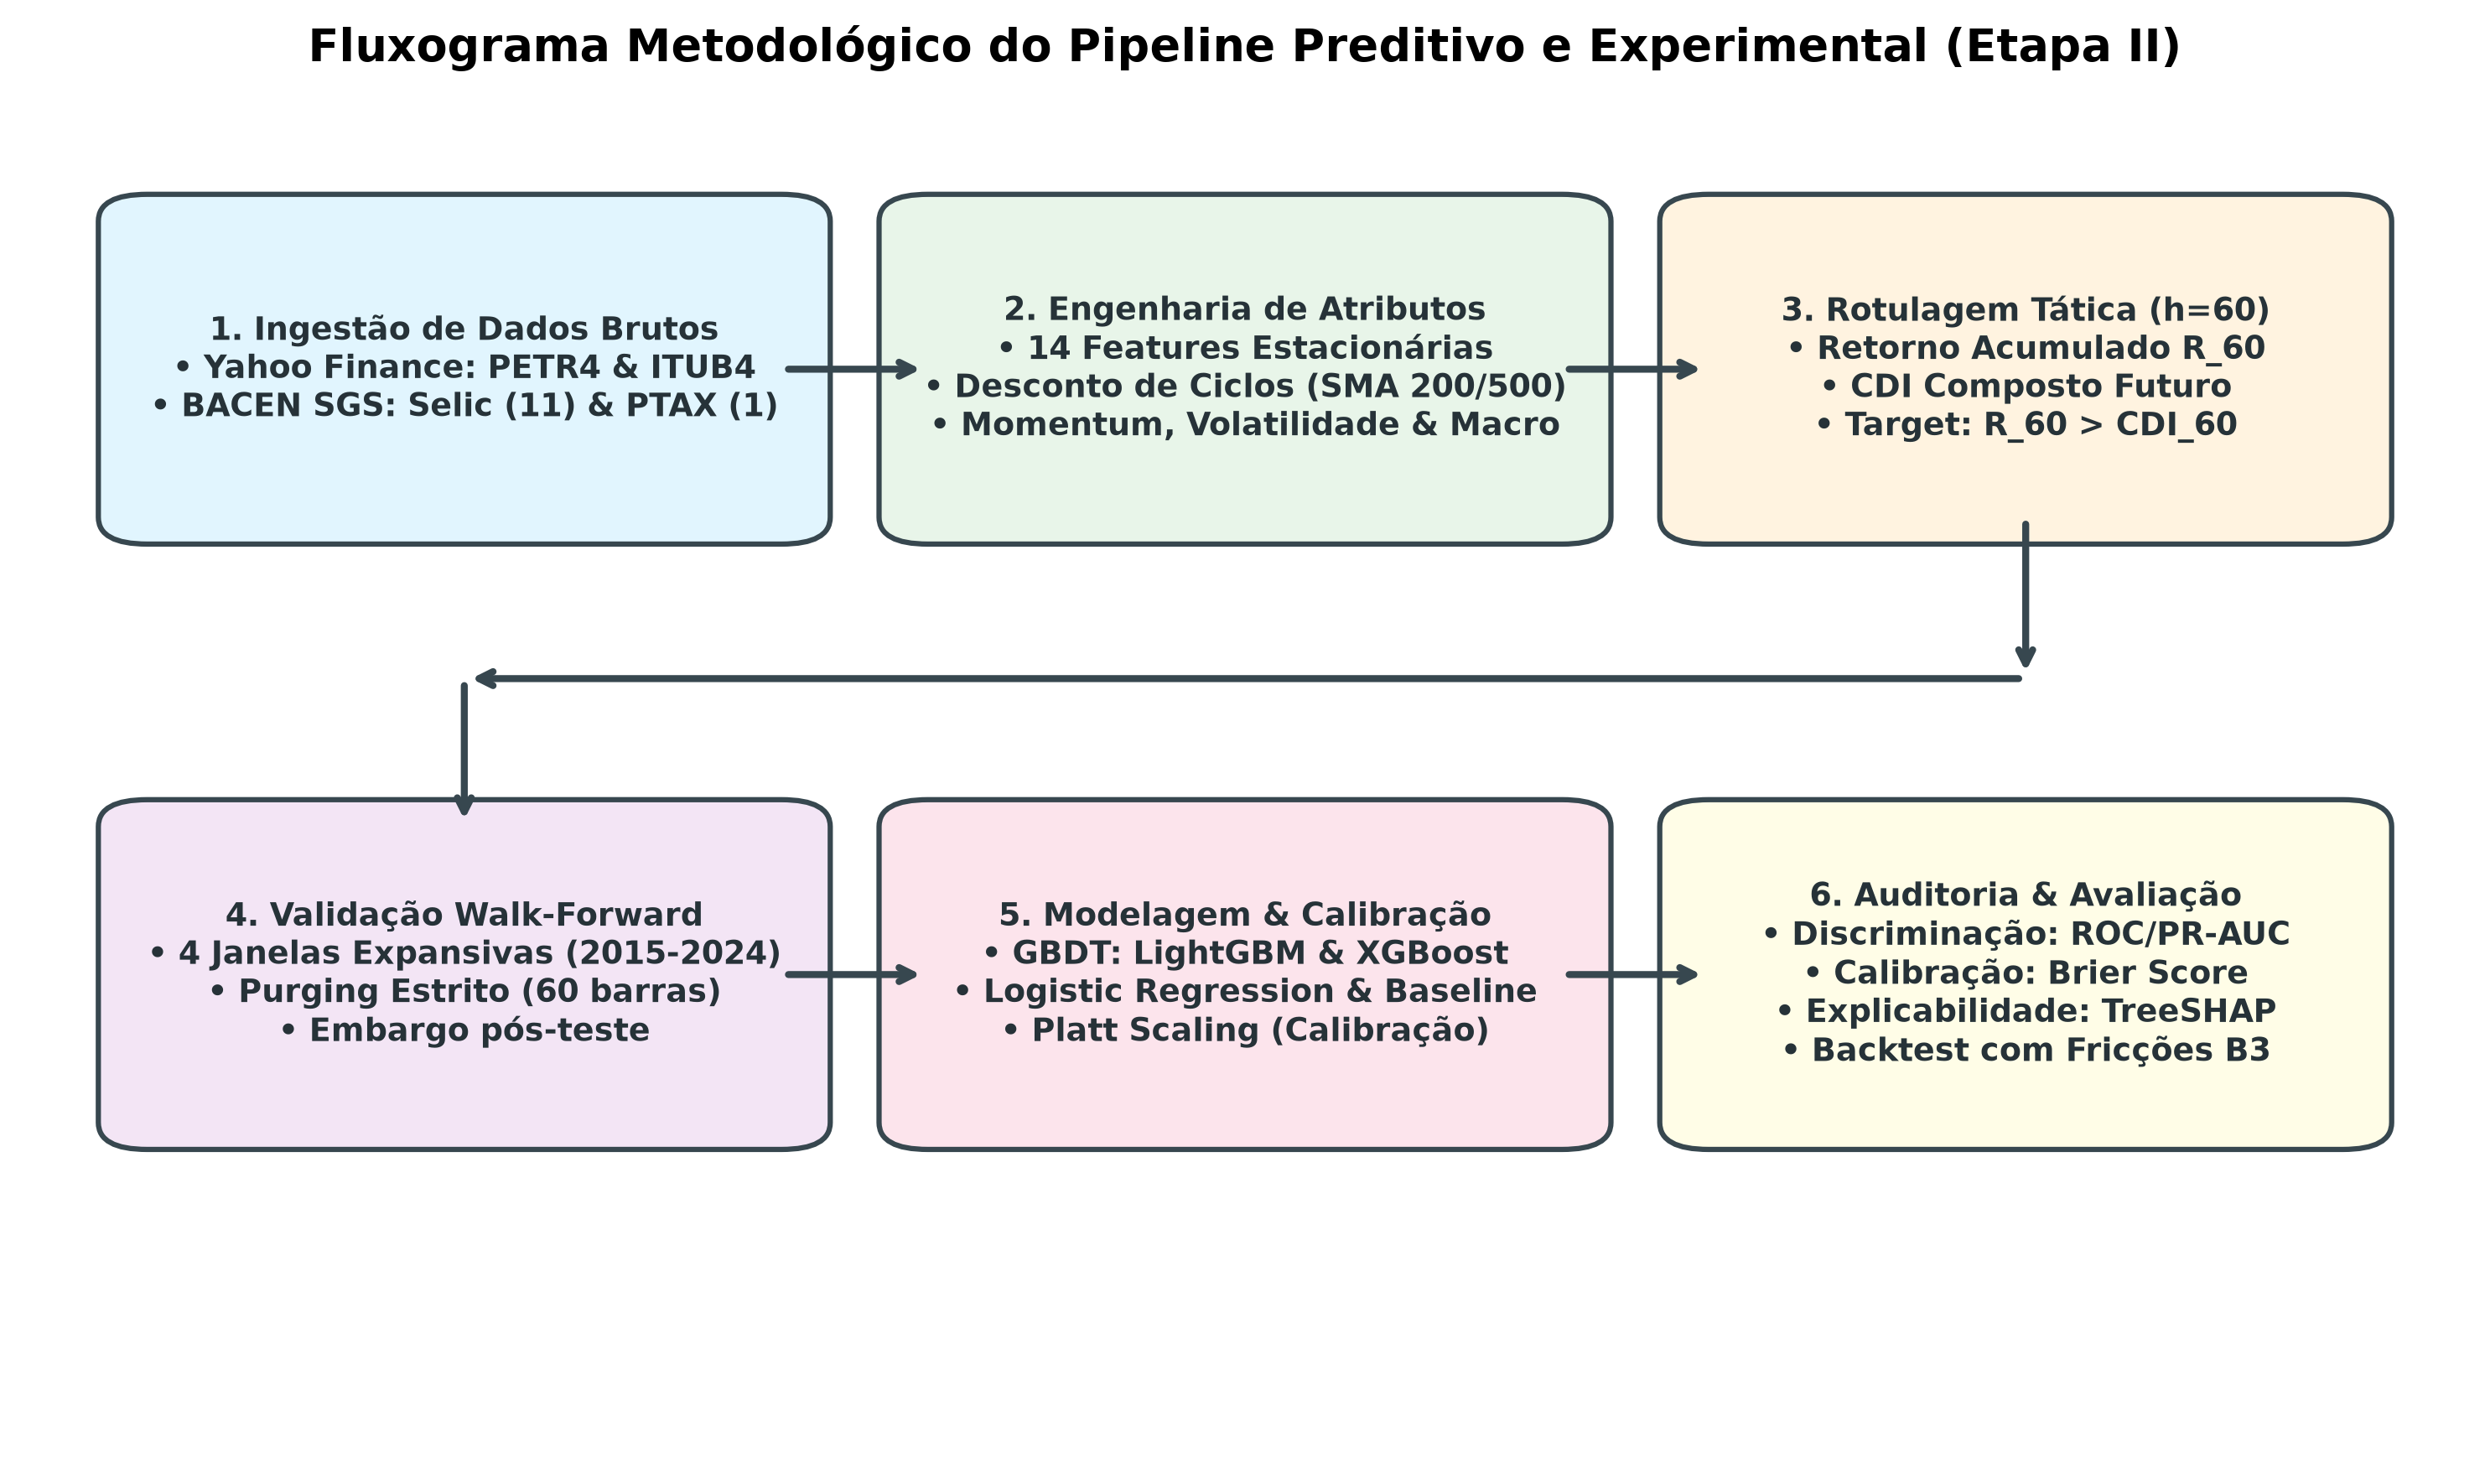
\includegraphics[width=0.48\textwidth]{figures/fluxograma_metodologia.png}
\caption{Fluxograma metodológico do pipeline preditivo e experimental (Etapa II).}
\label{fig:fluxograma}
\end{figure}

\bibliographystyle{IEEEtran}
\bibliography{references}

\end{document}
